\chapter{Results}
In this section, the results of the project will be discussed.

\section{System Integration}
This section details the physical system and the integration of the hardware. This includes power consumption, system layout, and component failures or difficulties. The system diagram shown in Figure \ref{masdr_system_diagram} will be explained in detail in this section.
\begin{figure}[ht!]
	\centering
	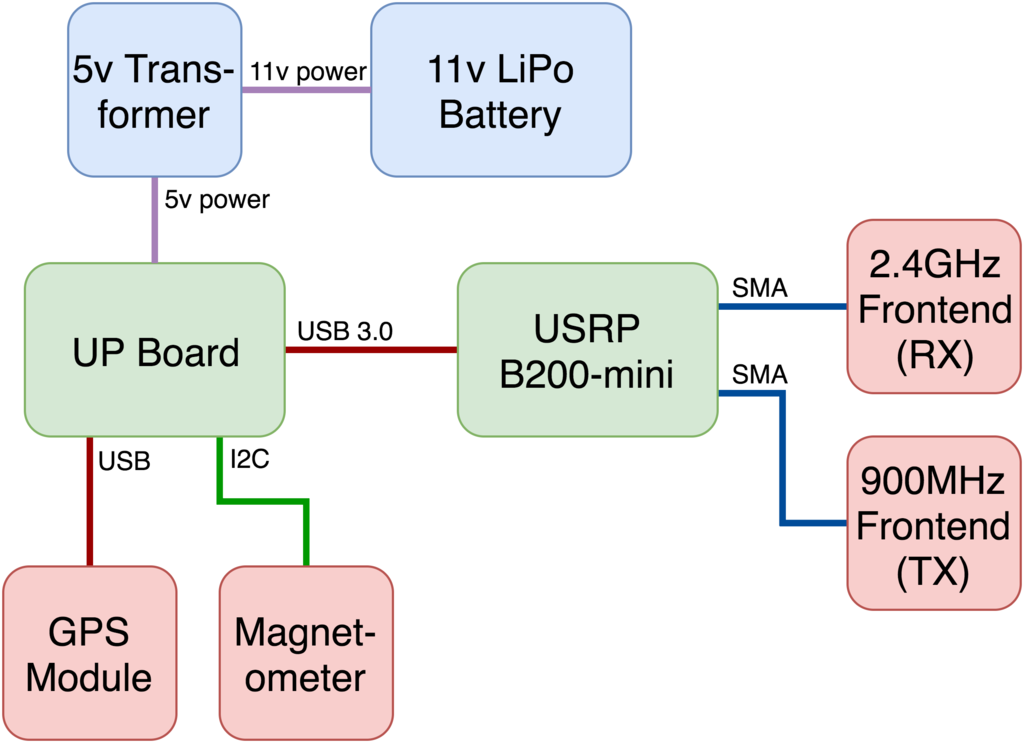
\includegraphics[width=0.70\textwidth]{img/masdr_system_diagram.png}
	\caption{MASDR system diagram detailing the connections between each component.}
	\label{fig:masdr_system_diagram}
\end{figure}\par
The encasing for the system was designed in SOLIDWORKS. It was fabricated using wood panels and a laser cutter. The encasing was designed to be as minimal as possible to reduce the weight of the system. This was done by cutting holes in the panels to remove as much material as possible and using metal supports instead of wooden walls. The metal supports were used in each of the corners to connect the two wooden panels as seen in Figure \ref{fig:connectors}.
\begin{figure}[ht!]
	\centering
	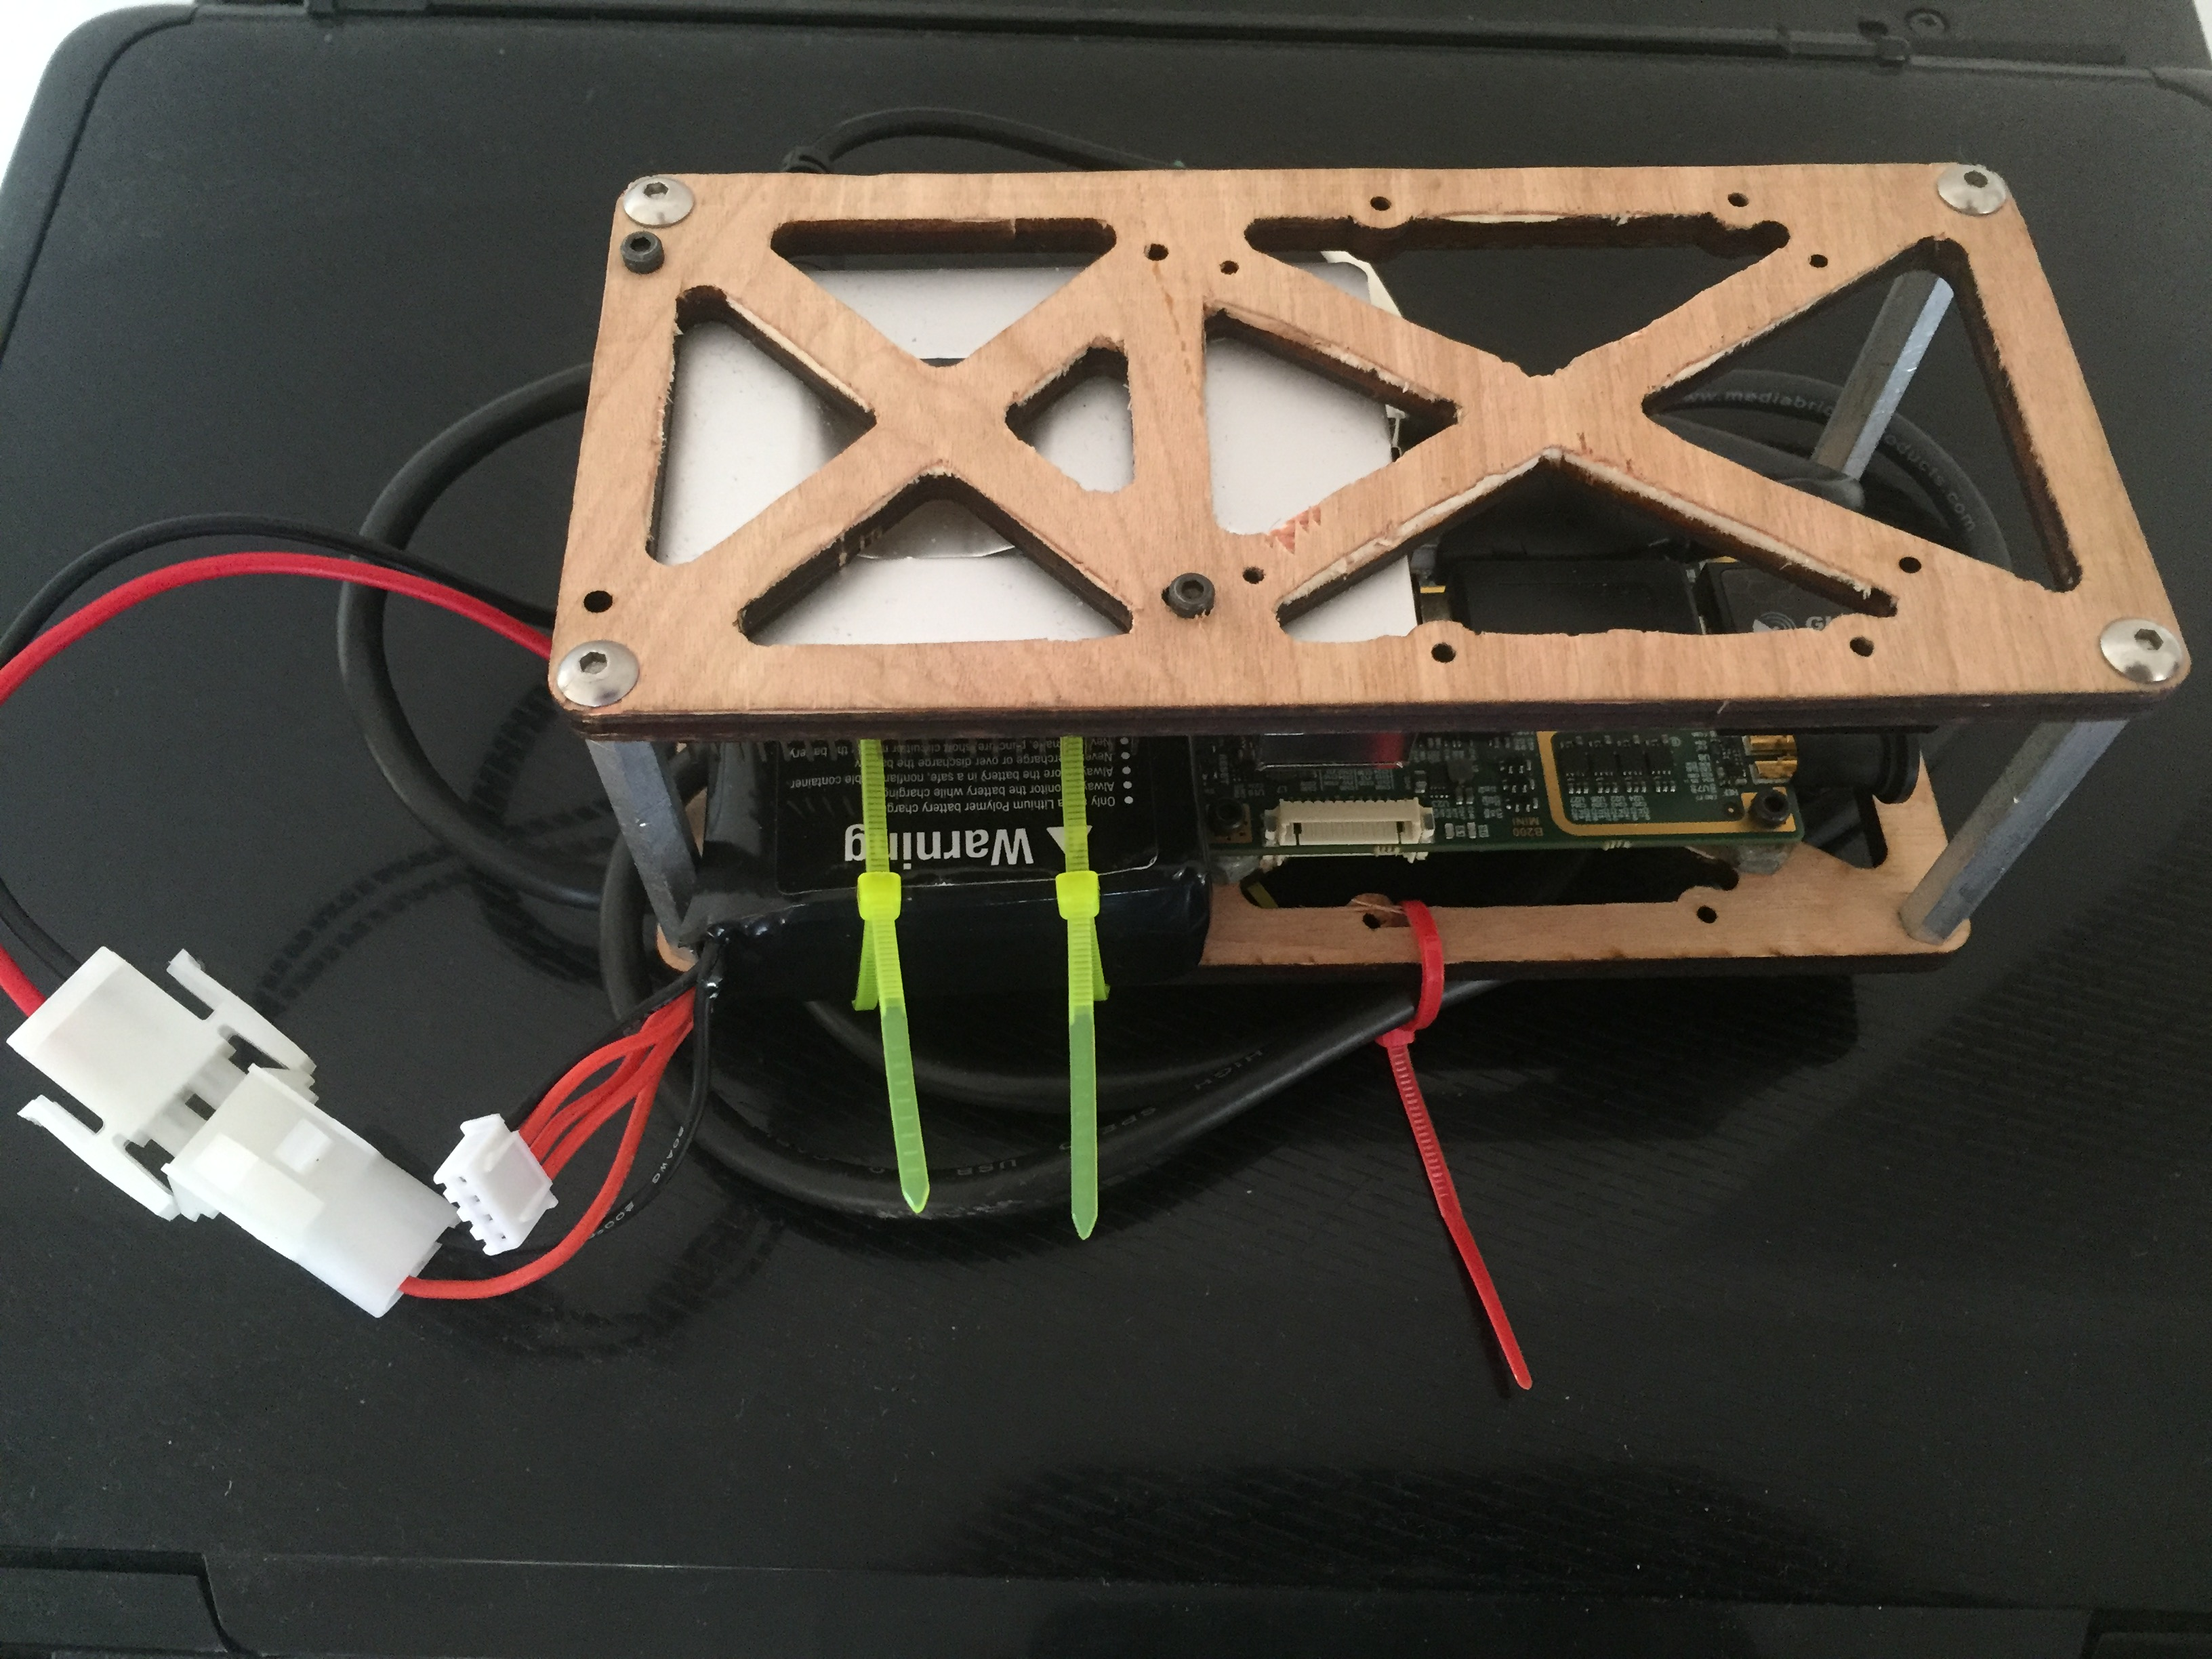
\includegraphics[width=0.70\textwidth]{img/Overhead_of_box.JPG}
	\caption{Overhead view of the encasing of the MASDR system}
	\label{fig:overhead_of_box}
\end{figure}\par
The two wooden panels were created identically to reduce design time and fabrication time. Screw holes were precut into the wood to ensure mounting the components wouldn't split the wood. This enclosure was mounted to the bottom of the drone using the hardware mount on the drone detailed in Section \ref{Mounting}. \par

To power the system, an 11V LiPo battery was used in combination with a 5V transformer to step down the voltage for use by the UP Board. The battery and converter were connected using connectors seen in Figure \ref{fig:connectors}, so that the battery could be disconnected when it is not in use. The male connector was soldered to the transformer and the female connector was soldered to the battery.
\begin{figure}[ht!]
	\centering
	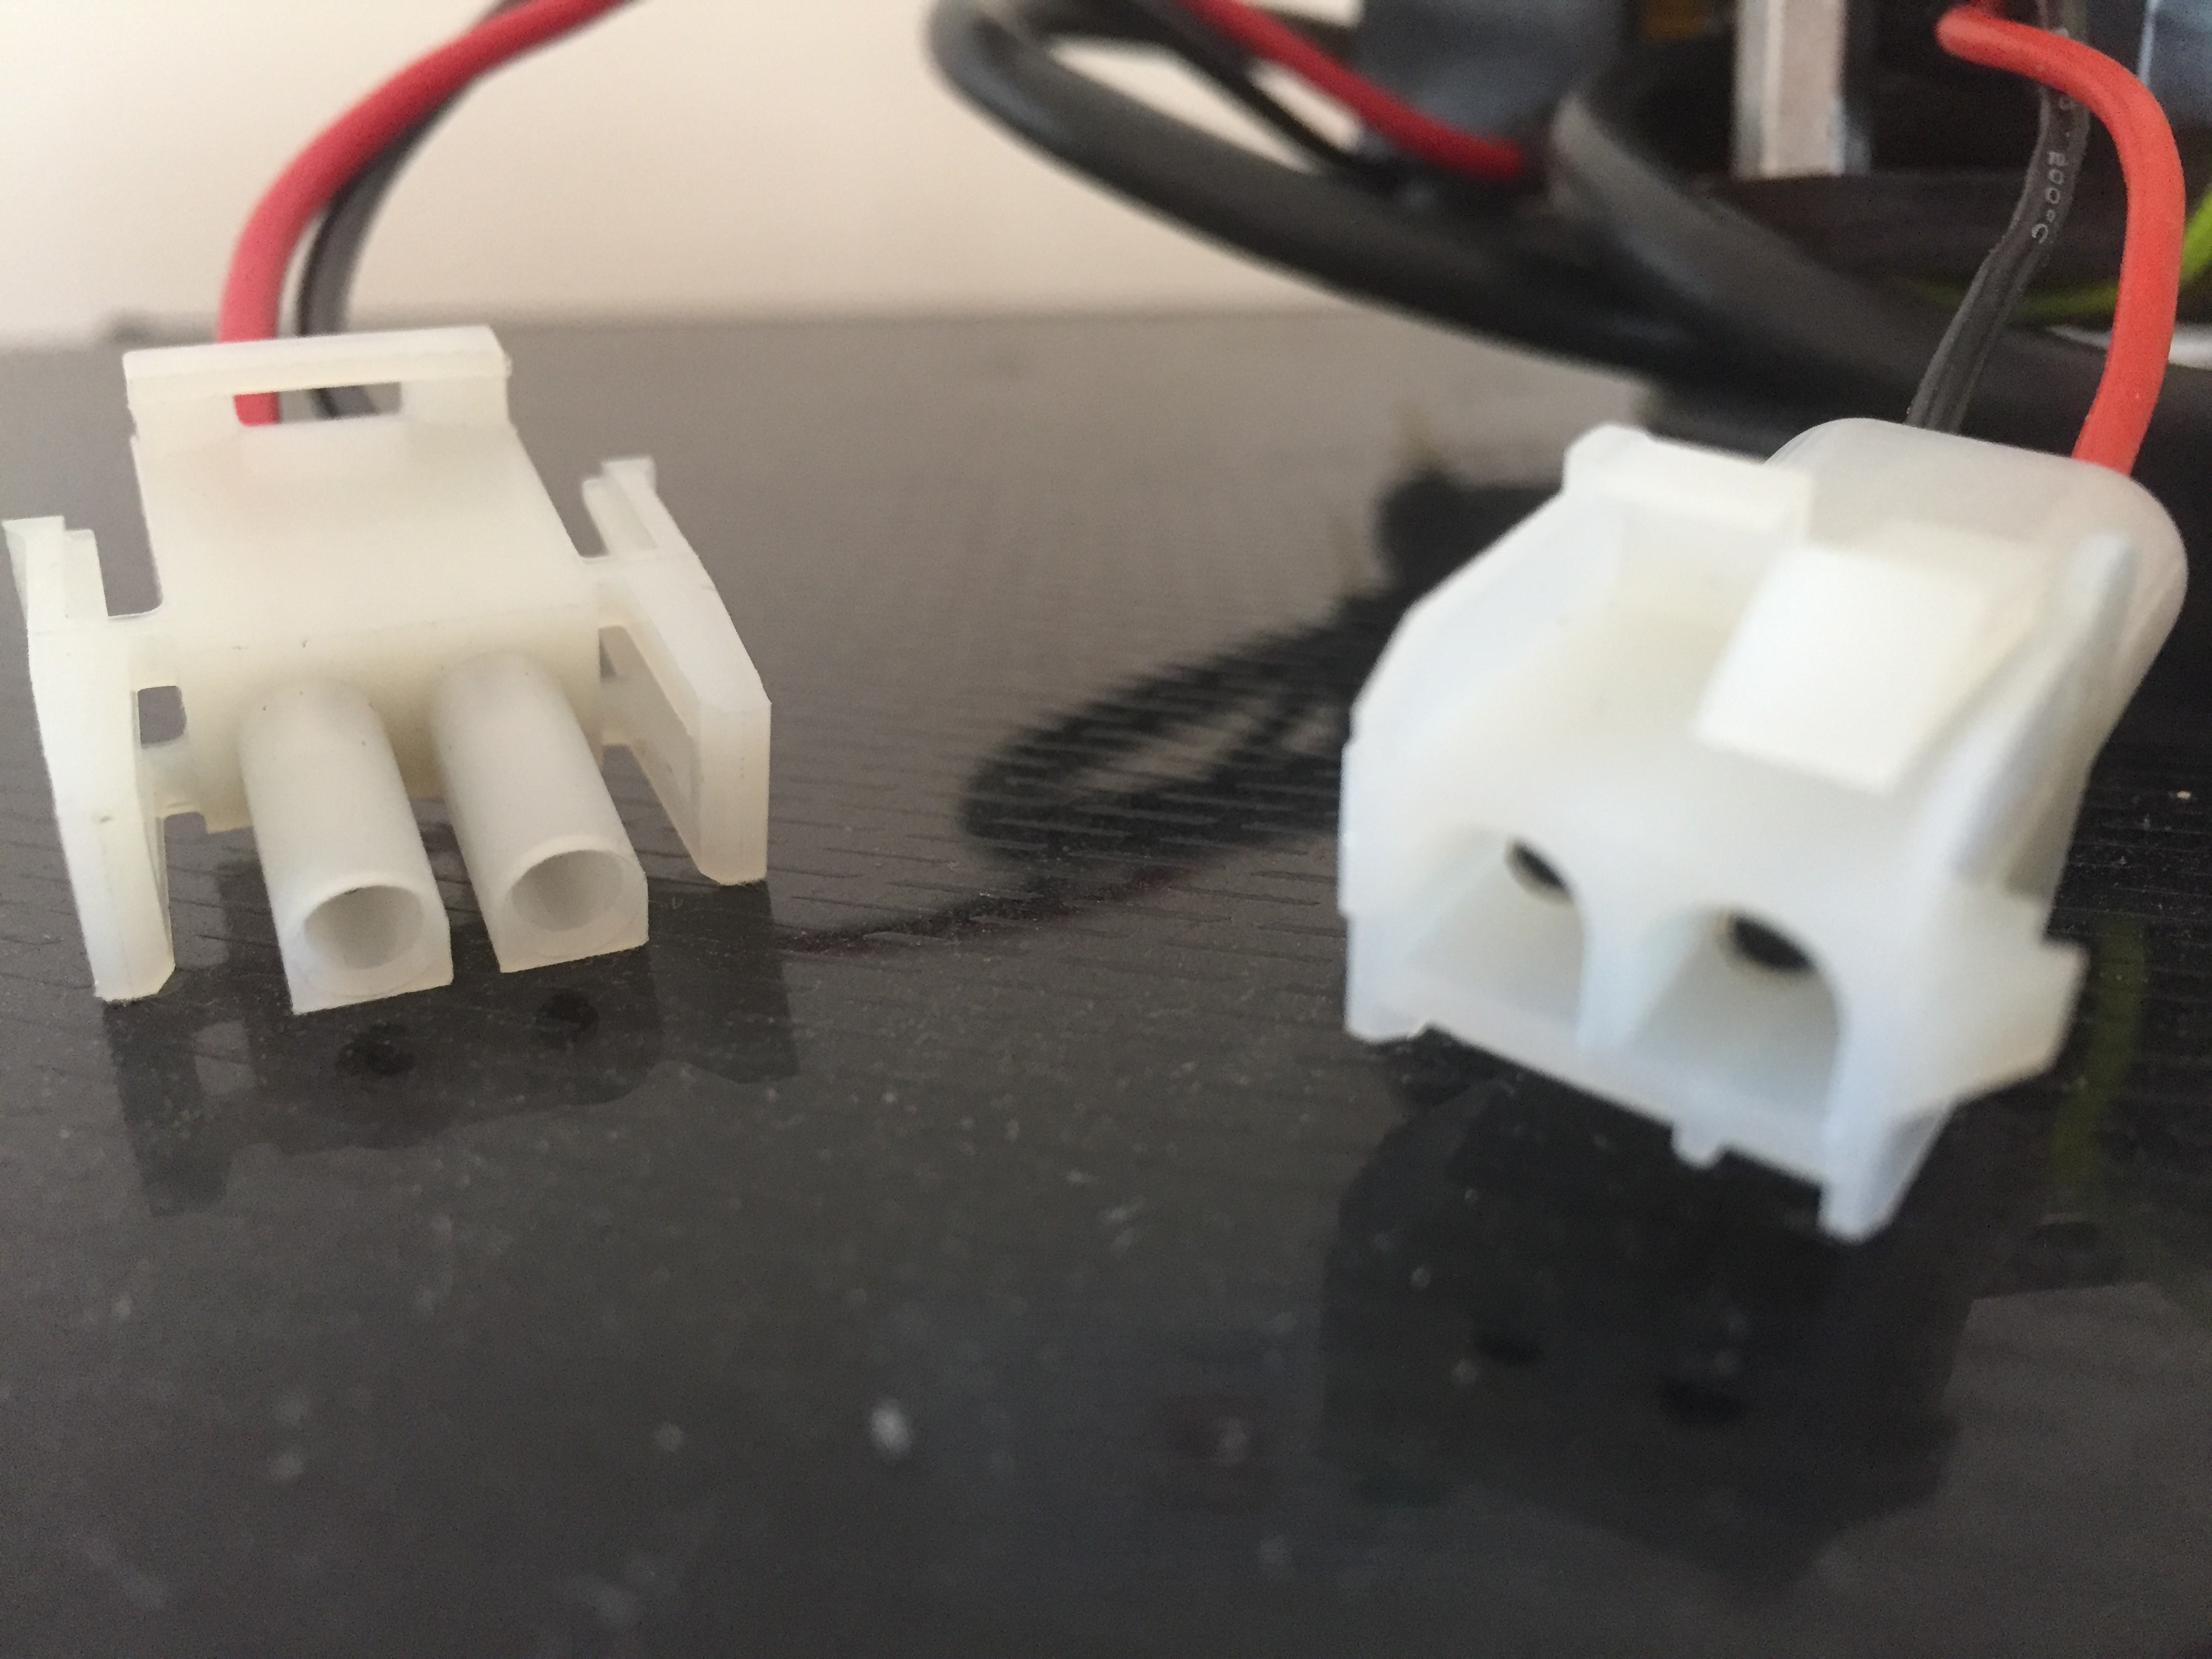
\includegraphics[width=0.70\textwidth]{img/connectors.JPG}
	\caption{Connectors for the battery. The male connector (left) is connected to the transformer and the female connector (right) is connected to the LiPo battery.}
	\label{fig:connectors}
\end{figure}\par
The first transformer that was used in the system failed because it became disconnected from the UP Board when power was applied. This transformer was a buck converter which can fail when an output isn't connected because of the failure of a MOSFET or diode. A new transformer was purchased to replace the malfunctioning one. \par

The UP Board is connected to the 5V transformer using a barrel jack. The male connector was soldered onto the output of the transformer. The UP Board is the main system with everything else connected to it through USB or I2C. It was mounted upside down on the top panel as shown in Figure \ref{fig:box_usb_view}.
\begin{figure}[ht!]
	\centering
	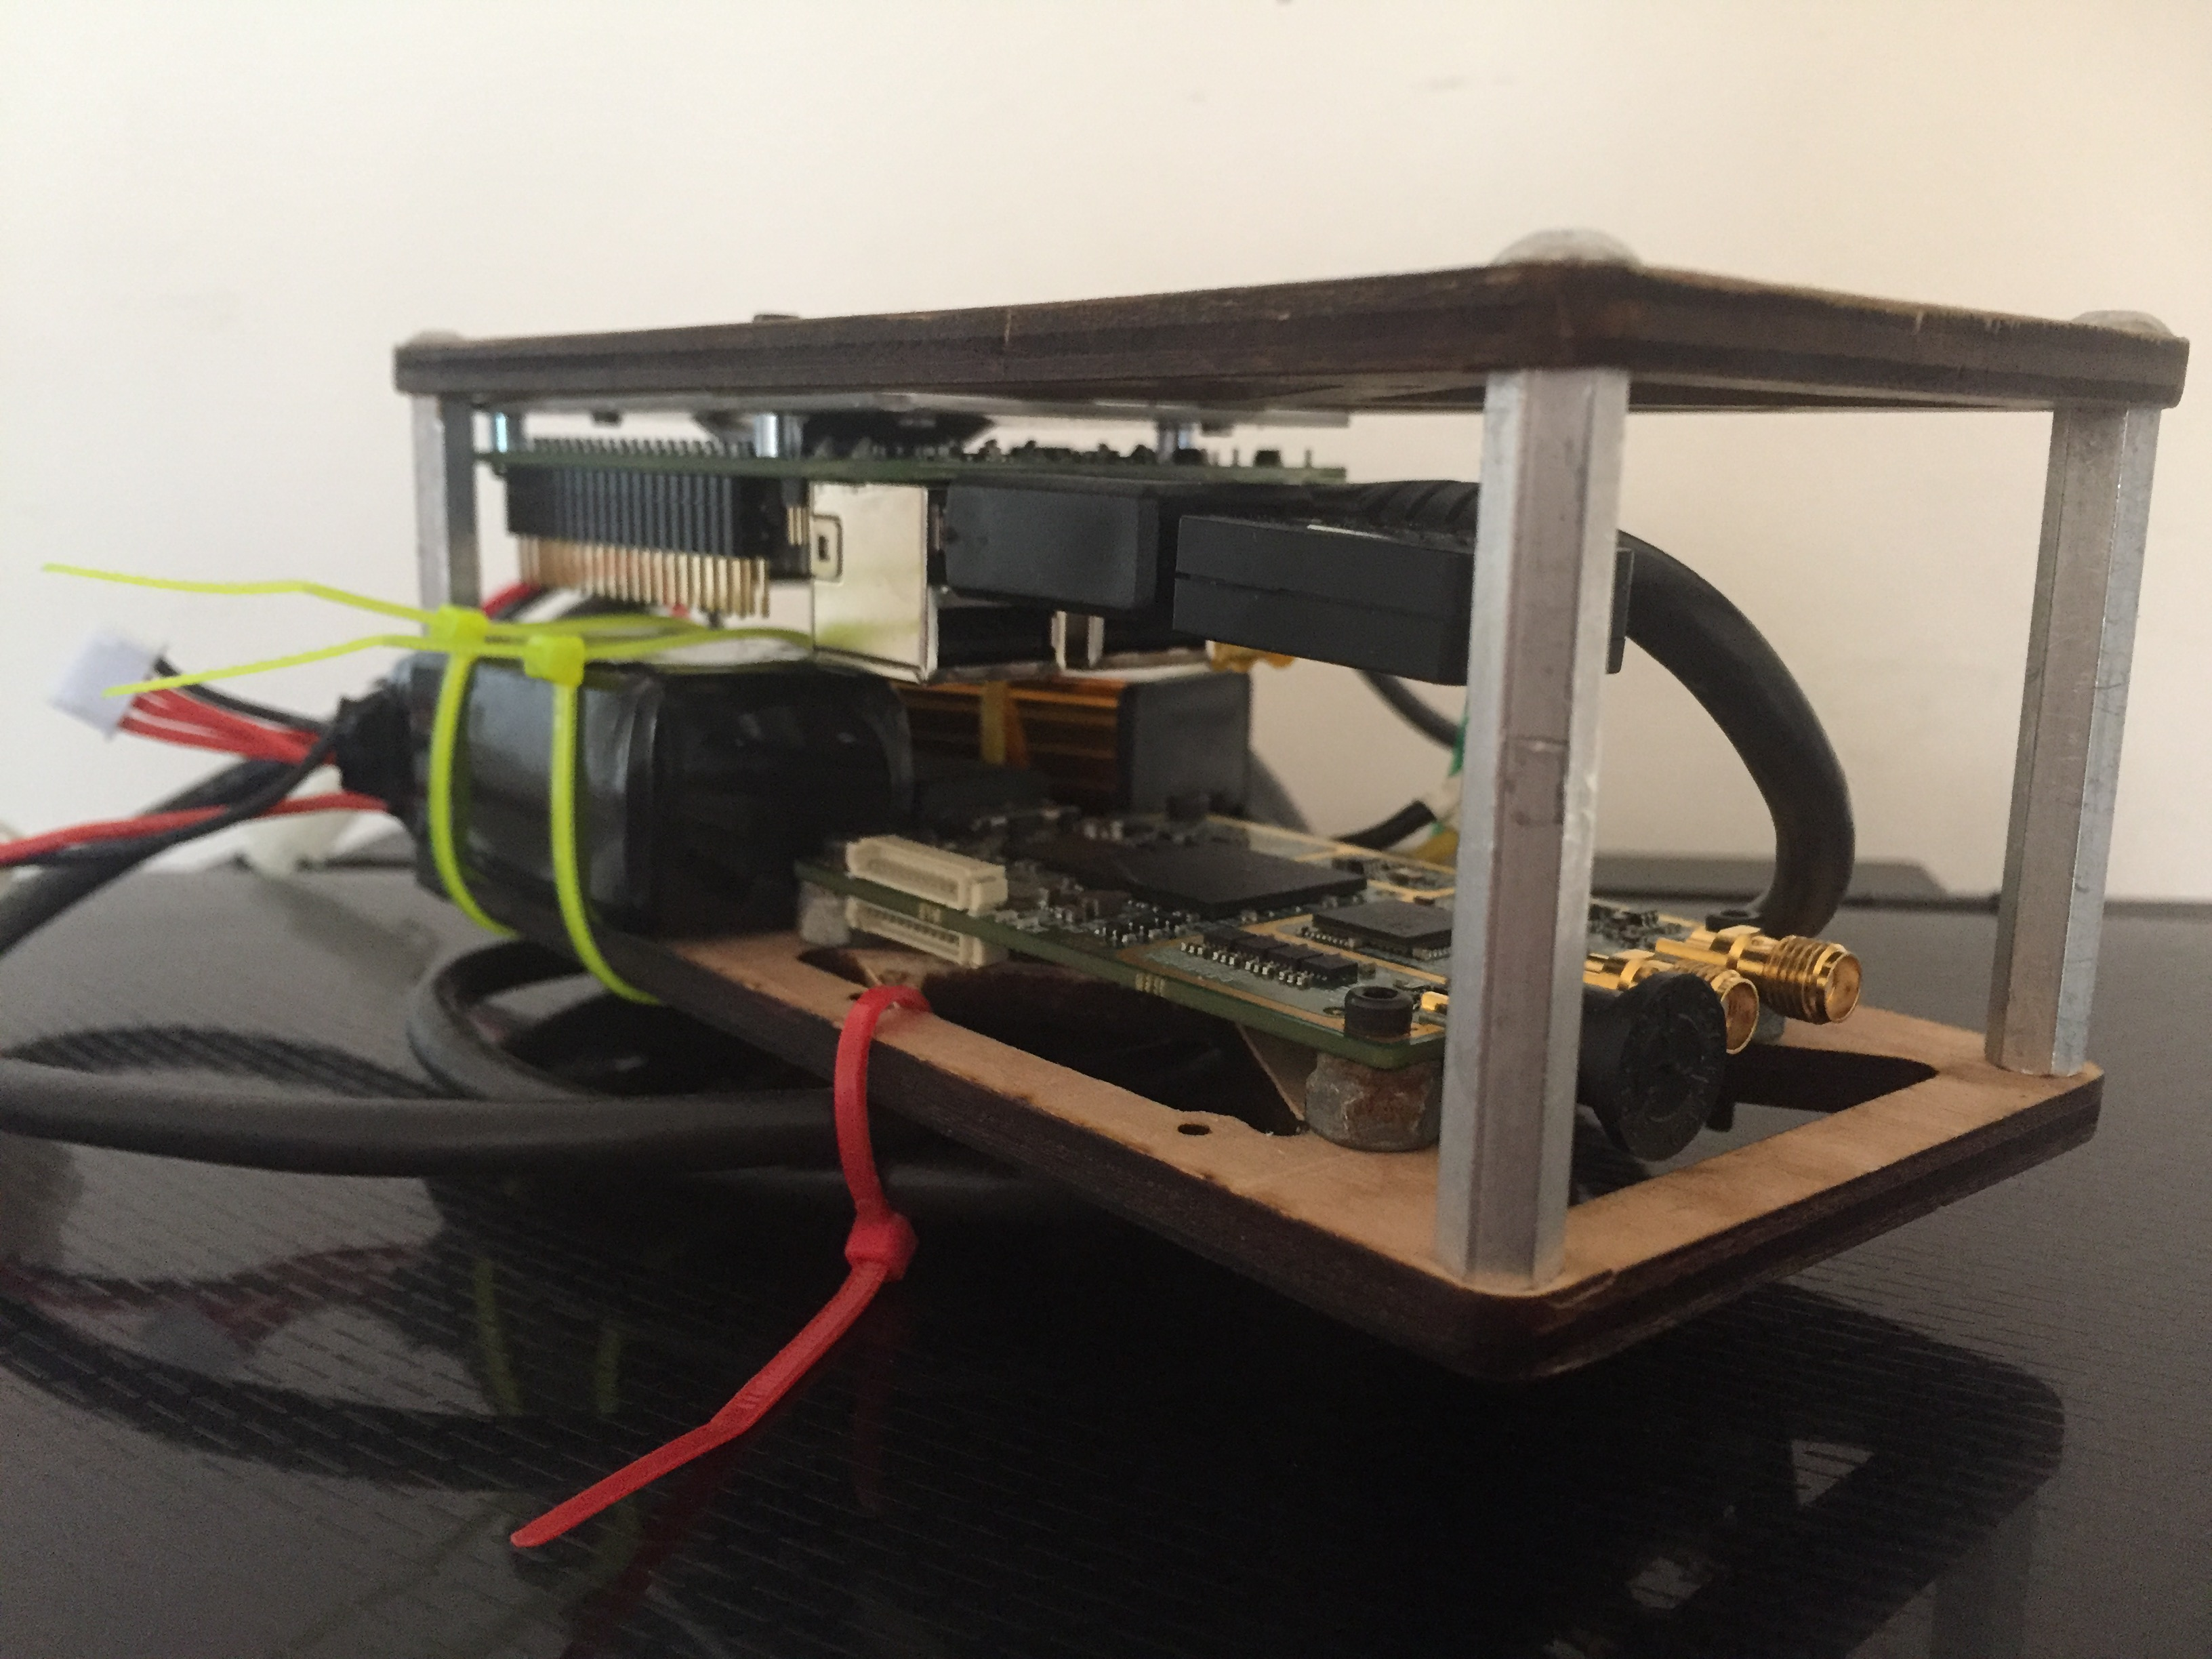
\includegraphics[width=0.70\textwidth]{img/box_usb_view.JPG}
	\caption{Angled side view of the encasing with the UP Board connected to the top panel with the GPS and USB cable to the B200-Mini. The golden transformer and the battery are positioned directly under the UP Board on the bottom panel. The B200-Mini is connected to the bottom panel and is the closes board to the camera.}
	\label{fig:box_usb_view}
\end{figure}\par
The GPS is connected to the UP Board using an micro USB to USB adapter. Integration and operation of the GPS proved to be a challenge. The GPSD library that was used to interface with the GPS had permission issues that caused the GPS data to not be read by a C++ program. After the permissions were set correctly, the MASDR program was able to correctly read the GPS data.\par

The magnetometer was to be connected to the UP Board using the I2C pins. Communication between the UP Board and the magnetometer was never established after multiple attempts. The UP Board would send a signal to the magnetometer, but never received a response. This could be due to a lack of a Linux driver or a faulty board. A Linux driver for the magnetometer wasn't provided by the manufacturer and the time line of the project made it unfeasible to write a driver by hand.\par

The B-200 mini was attached to the bottom panel of the casing. It communicated to the UP Board through a wired USB connection. The 900MHz and 2.4GHz antennas were connected to the SMA connectors on the mini. The 2.4GHz antenna required an adapter because the connector on the board was a smaller size than the one on the antenna. During testing, it was realized that the transmission from the board was not working. Upon further inspection it was noticed that a component had broken off the board. Another board was borrowed from a lab to verify that the original board was faulty. The transmission test ran successfully on the board from the lab. A working board and the broken board are shown in the Figure \ref{fig:working_mini} and Figure \ref{fig:broken_mini} respectively.
\begin{figure}[ht!]
	\centering
	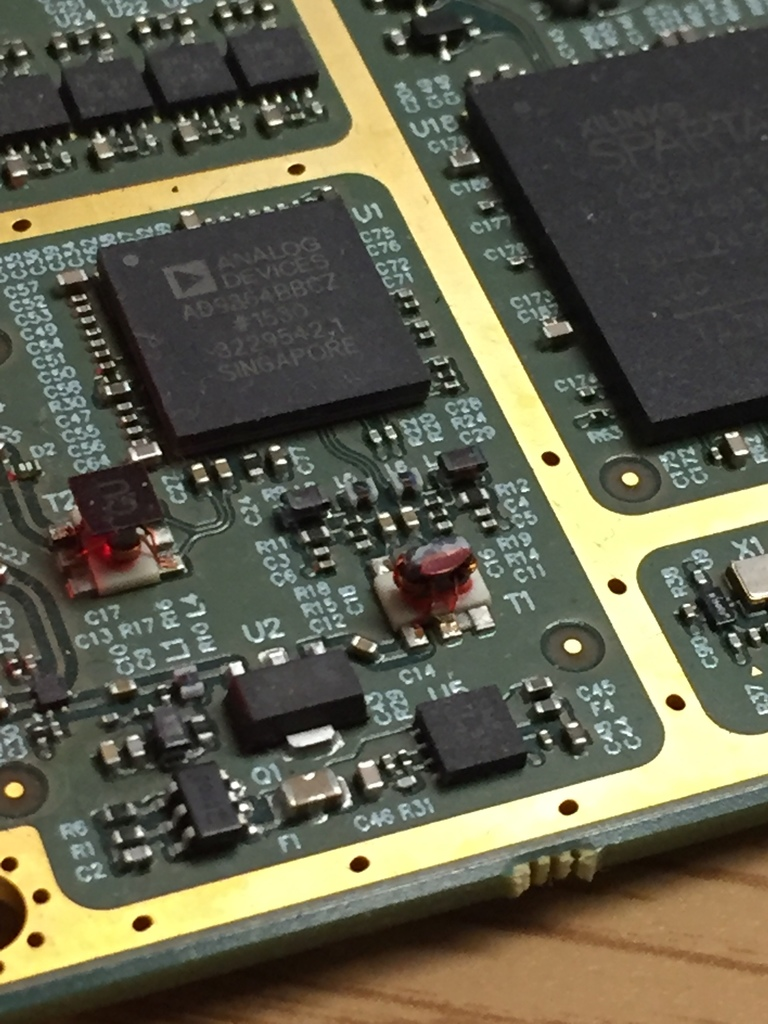
\includegraphics[width=0.70\textwidth]{img/working_mini.jpg}
	\caption{The functional B200-mini}
	\label{fig:working_mini}
\end{figure}\par
\begin{figure}[ht!]
	\centering
	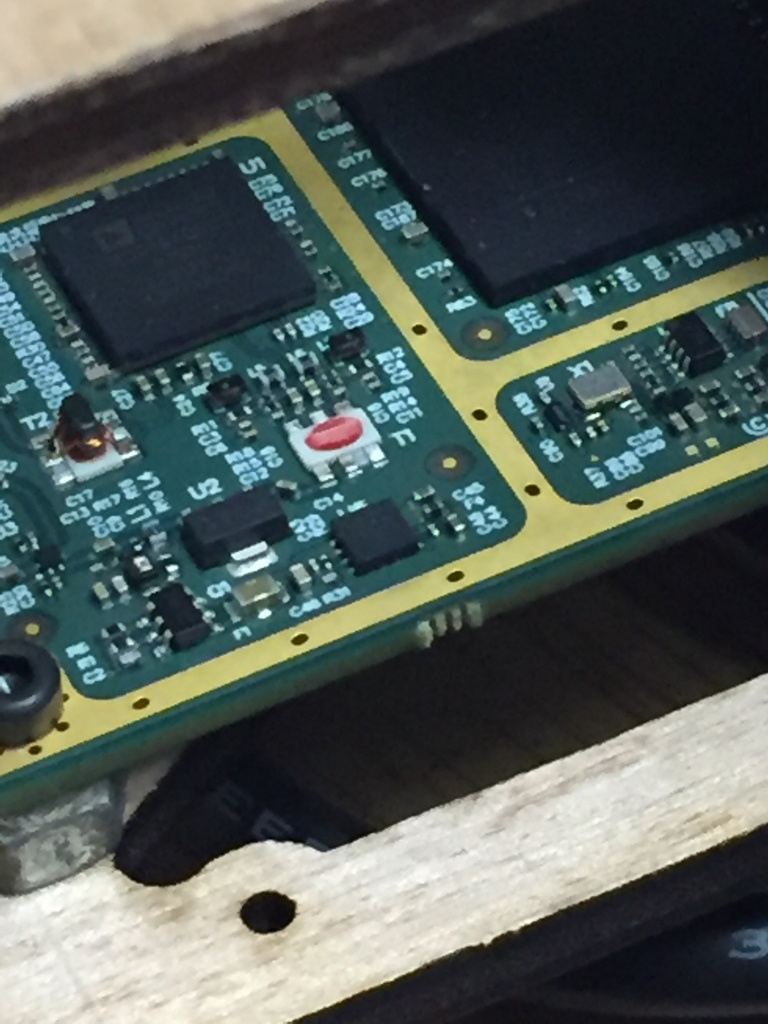
\includegraphics[width=0.70\textwidth]{img/broken_mini.jpg}
	\caption{The non-functional B200-mini}
	\label{fig:broken_mini}
\end{figure}\par
This component may have broken off during transport to and from meetings or because of vibrations during in flight testing. \par

The complete system mounted on the drone is shown in Figure \ref{fig:drone_and_box}.
\begin{figure}[ht!]
	\centering
	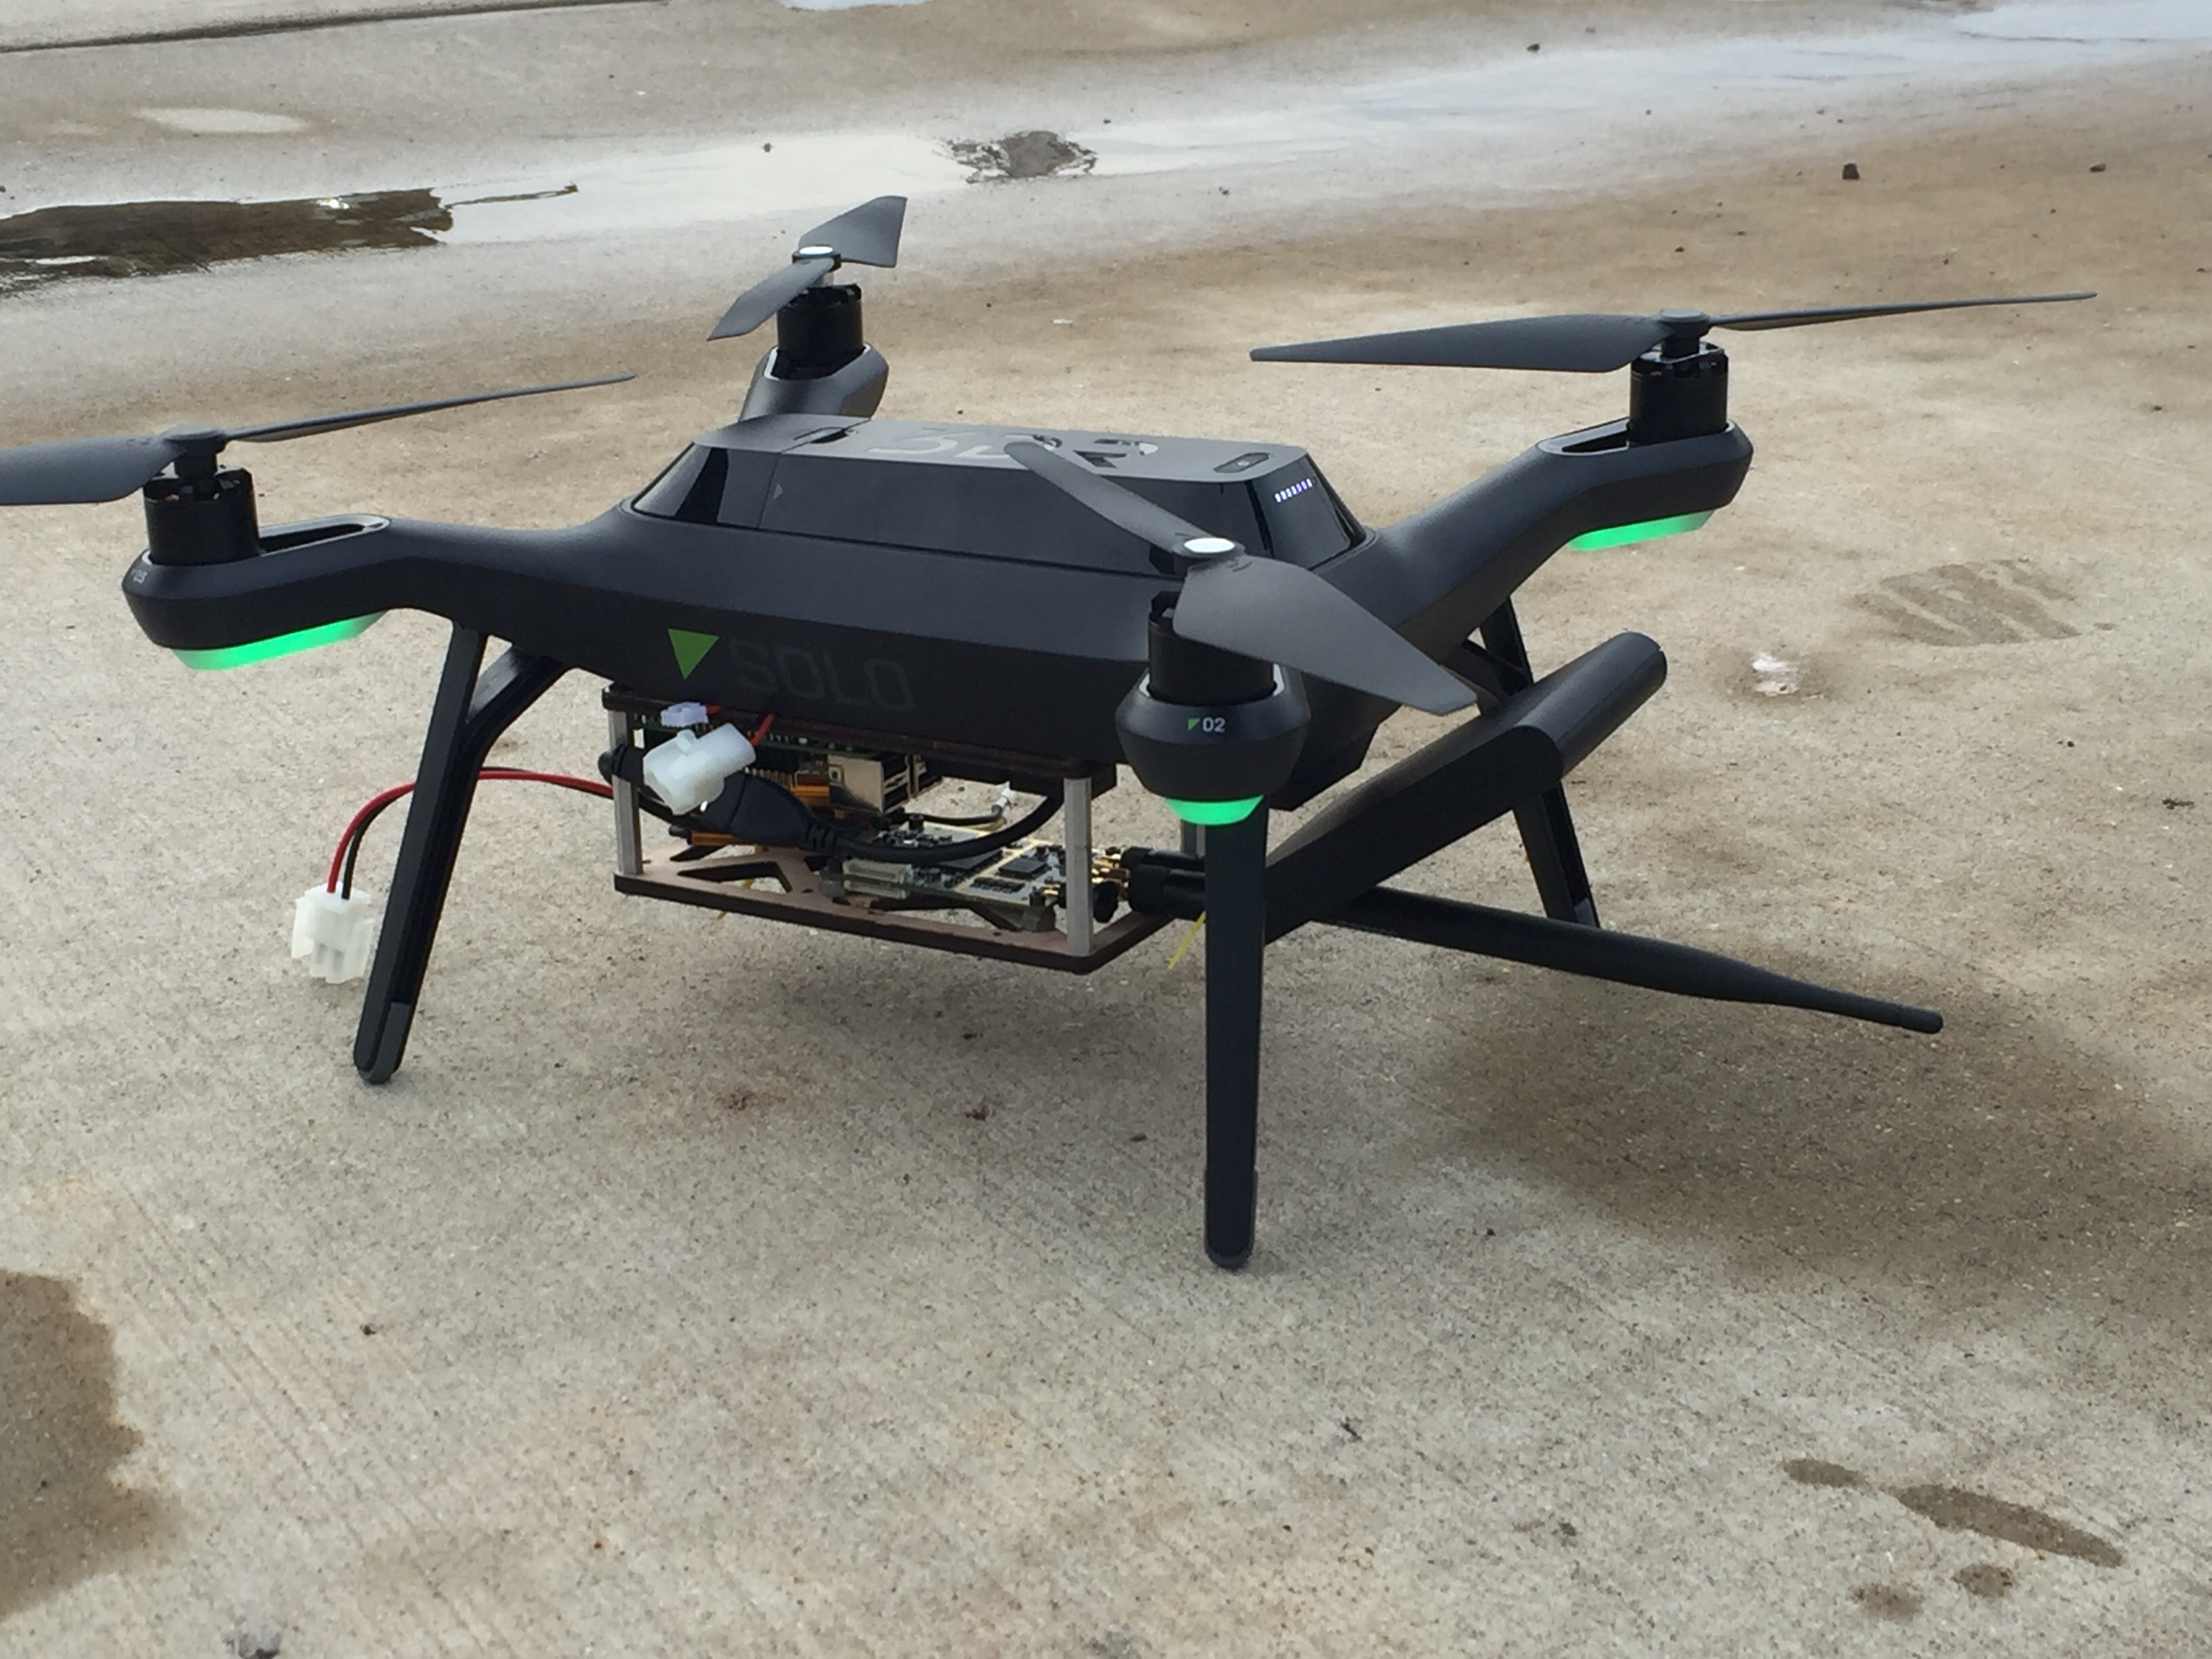
\includegraphics[width=0.70\textwidth]{img/drone_and_box.jpg}
	\caption{The complete system mounted on the drone. In flight testing was done with this setup.}
	\label{fig:drone_and_box}
\end{figure}\par

\section{Code Framework}
\section{Drone Control}
\section{Spectrum Sensing}
In addition to calculating RSS values, a C++ program separate from the code framework
was written. This program, called iq\_to\_file, was created as a foundation with 
which to work with. It became the testbed for specific elements of MASDR, since it
was already capable of logging.The code for this section is in Appendix \ref{app:iq_to_file}. 
This program is built on the rx_samples_to_file example that Ettus Research provides 
with the UHD. This program already had the desired base functionality, so it proved
to be a good starting point. The program was then stripped of unnecessary functionality,
including the command-line interface. \par

\section{Spectrum Localization}
\section{Transmit To Ground}
\section{Summary}
